%%%%%%%%%%%%%%%%%%%% author.tex %%%%%%%%%%%%%%%%%%%%%%%%%%%%%%%%%%%
%
% sample root file for your "contribution" to a proceedings volume
%
% Use this file as a template for your own input.
%
%%%%%%%%%%%%%%%% Springer %%%%%%%%%%%%%%%%%%%%%%%%%%%%%%%%%%


\documentclass{svproc}
%
% RECOMMENDED %%%%%%%%%%%%%%%%%%%%%%%%%%%%%%%%%%%%%%%%%%%%%%%%%%%
%

% to typeset URLs, URIs, and DOIs
\usepackage{url}
\usepackage{graphicx}
\usepackage{tabularx}
\setlength{\extrarowheight}{6pt}
\usepackage{enumitem}

\begin{filecontents}{citace.bib}
@inproceedings{kruuza2012making,
  title={Making Community and ASR Join Forces in Web Environment},
  author={Kr\r{u}za, Old{\v{r}}ich and Peterek, Nino},
  booktitle={International Conference on Text, Speech and Dialogue},
  pages={415--421},
  year={2012},
  organization={Springer}
}
@article{codd1970relational,
  title={A relational model of data for large shared data banks},
  author={Codd, Edgar F},
  journal={Communications of the ACM},
  volume={13},
  number={6},
  pages={377--387},
  year={1970},
  publisher={ACM}
}
@article{adenot2013web,
  title={Web audio api},
  author={Adenot, Paul and Wilson, Chris and Rogers, Chris},
  journal={W3C, October},
  volume={10},
  year={2013}
}
@article{mihalcea2004building,
  title={Building sense tagged corpora with volunteer contributions over the web},
  author={Mihalcea, Rada and Chklovski, Timothy},
  journal={Recent Advances in Natural Language Processing III: Selected Papers from RANLP 2003},
  volume={260},
  pages={357},
  year={2004},
  publisher={John Benjamins Publishing}
}
@article{abramov2015redux,
  title={Redux},
  author={Abramov, D},
  journal={React Community, c},
  year={2015}
}
@article{hajek2007cesky,
  title={\v{C}esk\'{y} mystik Karel Mako\v{n}},
  author={Jurik H\'{a}jek},
  journal={Dingir},
  year={2007},
  volume={2007/4},
  pages={142--143},
  publisher={Dingir, s.r.o.},
  ISSN={1212-1371},
  editor={Zden\v{e}k Vojt\'{i}\v{s}ek}
}
@inproceedings{ide2010manually,
  title={The manually annotated sub-corpus: A community resource for and by the people},
  author={Ide, Nancy and Fellbaum, Christiane and Baker, Collin and Passonneau, Rebecca},
  booktitle={Proceedings of the ACL 2010 conference short papers},
  pages={68--73},
  year={2010},
  organization={Association for Computational Linguistics}
}
@article{bojar2008czeng,
  title={CzEng 0.7: Parallel Corpus with Community-Supplied Translations},
  author={Bojar, Ond{\v{r}}ej and Jan{\'\i}{\v{c}}ek, Miroslav and {\v{C}}e{\v{s}}ka, Pavel and Be{\v{n}}a, Peter and others},
  journal={LREC 2008},
  year={2008}
}
@inproceedings{5494979,
  author={M. Marge and S. Banerjee and A. I. Rudnicky},
  booktitle={2010 IEEE International Conference on Acoustics, Speech and Signal Processing},
  title={Using the Amazon Mechanical Turk for transcription of spoken language},
  year={2010},
  volume={},
  number={},
  pages={5270-5273},
  keywords={linguistics;natural language processing;speech processing;Amazon mechanical turk service;MTurk marketplace;Rover voting scheme;speaker demographics;spoken language transcription;transcription guideline;Computer science;Costs;Demography;Gold;Guidelines;Humans;Natural languages;Recruitment;Speech synthesis;Streaming media;crowd sourcing;speech transcription},
  doi={10.1109/ICASSP.2010.5494979},
  ISSN={1520-6149},
  month={March},
}
@article{reese2010wikicorpus,
  title={Wikicorpus: A word-sense disambiguated multilingual wikipedia corpus},
  author={Reese, Samuel and Boleda, Gemma and Cuadros, Montse and Rigau, German},
  year={2010},
  publisher={Citeseer}
}
\end{filecontents}


\def\UrlFont{\rmfamily}

\begin{document}
\mainmatter              % start of a contribution
%
\title{Second-Generation Web Interface to Correcting ASR Output}
%
\titlerunning{Second-Generation Web Interface to Correcting ASR Output}  % abbreviated title (for running head)
%                                     also used for the TOC unless
%                                     \toctitle is used
%
\author{Old\v{r}ich Kr\r{u}za and Vladislav Kubo\v{n}}
%
\authorrunning{Kr\r{u}za, Kubo\v{n}} % abbreviated author list (for running head)
%
%%%% list of authors for the TOC (use if author list has to be modified)
%\tocauthor{Ivar Ekeland, Roger Temam, Jeffrey Dean, David Grove,
%Craig Chambers, Kim B. Bruce, and Elisa Bertino}
%
\institute{Charles University\\
           Faculty of Mathematics and Physics\\
           Institute of Formal and Applied Linguistics\\
           Malostransk\'{e} n\'{a}m. 25, Prague, Czech Republic\\
           \{kruza,vk\}@ufal.mff.cuni.cz}

\maketitle              % typeset the title of the contribution

\begin{abstract}
This paper presents a next-generation web application that enables users to
contribute corrections to automatically acquired transcription of long speech
recordings. We describe differences from similar settings, compare our solution
with others and reflect on the development from the now 6 years old work we
build upon in the light of the progress made, lessons learned and the new
technologies available in the browser.
\keywords{Speech recognition, transcription, community-driven, web standards}
\end{abstract}

\section{Introduction}

In 2012\cite{kruuza2012making}, we have presented a setting where a community of
users contributed corrections to automatically transcribed talks of a single
speaker. Now that the browser technologies evolved drastically and we could
observe the usage patterns and discover shortcomings of the solution at hand, we
have created a next generation of the programme. We shall describe the steps
taken and discuss their motivation and impact.

The application we describe is a part of a larger system that deals with
Mako\v{n}'s recordings. It consists roughly of (1) the corpus itself, (2) an ASR
system trained specially for it and (3) a web interface for the users. These
three parts form a whole where the ASR gives a baseline transcription, the users
correct it and the corrections are fed as further training data to the acoustic
and language models. In this paper, we focus on the web interface.

\subsection{Motivation}

Our project focuses on the collection of recordings of Karel
Mako\v{n}\cite{hajek2007cesky} *1912 \textdagger1993, the author of numerous
books, translations and comments to works of spiritual and religious nature, who
was influenced by trances during recurring surgery without anesthesy in the age
of 6, ecstasies in the youth and finally facing and surviving certain death in a
Nazi concentration camp, after which he experienced enlightenment. He gave talks
in a narrow circle of friends and the recordings in our care have been taken
between early 70's and 1991, spanning about 1000 hours in total.

All of Mako\v{n}'s work deals more or less directly with a single topic:
entering the eternal life before the physical death. He draws mainly from the
Christian symbolism, builds up on Christian mysticism and ancient tradition of
India and China.

Mako\v{n}'s written works present his teachings in a systematic, comprehensive
fashion, while the recordings offer bonuses: talks tailored to the audience,
answers to questions, personal experiences, behind-the-scenes to the books etc.
The archive is freely
accessible\footnote{https://lindat.mff.cuni.cz/repository/xmlui/handle/11372/LRT-1455}
under the CC-BY license.

\section{Differences to Other Settings}

The spoken corpus is about 1000 hours of a single
speaker. Our aim is to have a transcription as good as possible for the purpose
of searching and further, higher-level processing of the data. There is a pool
of people interested in the talks, who on one hand are the force we can try to
employ and on the other hand are the consumers of our effort, our target group
so to speak.

The web application should therefore combine the two purposes: 1. serve its user
with making the content available in a manner as good as possible and 2. animate
the user to give as much and as high-quality contribution as possible.

To our best knowledge, there is no other project with a comparable setting.
However, we can compare single aspects found in other applications.

\subsection{Transcription Apps}
\label{ssec:diff:trans}

The best widespread match to our task is that of creating an application for
transcribing speech recordings. Let us compare the two tasks, pointing out the
main points of difference. For reference, we take (1)
Transcriber\footnote{trans.sourceforge.net}, a classical open-source program
written in TCL, (2) oTranscribe\footnote{otranscribe.com}, a free modern
web-based transcription tool and (3) Transcribe\footnote{transcribe.wreally.com}
a commercial web-based transcription tool.

The numbers in the bullet list below denote the programs our statement applies
to. For example, of the three only Transcriber allows speaker annotation, hence
there is only the number (1) standing at the second list item.

\noindent
\begin{tabularx}{\textwidth}{
    @{\hspace{1.5em}}% Space for left bullet
    >{{\hsize=0.9\hsize}\leavevmode\llap{\textbullet~}\raggedright}% Left bullet + formatting of column
    X% Left column specification
    @{\hspace{0.2em}}
    >{\hsize=0.2\hsize}
    X
    @{\quad\hspace{1.5em}}% Space between columns + right bullet space
    >{\leavevmode\llap{\textbullet~}\raggedright\arraybackslash}% Right bullet + formatting of column
    X% Right column specification
    @{}% No column space on right
  }
  \em{transcription applications}: & & \em{our application}: \\
  are optimized for the case where there is no transcription available and it
  must be acquired from scratch; &
    (1,2,3) &
      always assumes a prior transcription is available; \\

  allow annotation of speakers; &
    (1) &
      assumes all utterances come from the same speaker; \\

  need no quality control: the user is free to enter whatever transcription she
  pleases and the ultimate measure is her satisfaction; &
    (1,2,3) &
      needs the transcription to be accurate because it is used as training data
      for the acoustic model; \\

  use alignment on the level of phrases, if any; &
    (1)\footnote{
        Transcriber explicitly aligns the text with speech, while the
        other two merely support addition of timestamps into the transcription.
    } &
      uses alignment on the level of words; \\

  are user-centric: the user transcribes whatever acoustic data they choose; &
    (1,2,3) &
      is data-centric: the whole application with all its tools and persons
      revolves around the data set; \\

  assumes the user wants to transcribe; &
    (1,2,3) &
      assume the user wants to listen and possibly read along and we want to
      animate her to submit transcriptions; \\

  has no shared data between users; &
    (1,2)\footnote{Transcribe supports team co-operation.} &
      must count with collisions. \\
\end{tabularx}

\vspace{5mm}

Despite of these differences, we can still learn a lot from transcription
software. The ease of performing common tasks, like pausing, resuming and
rewinding is crucial for the user experience and in effect for the amount of
submissions that we receive. Also, the way the text is displayed synchronously
to the audio played has a big impact and the approaches have a lot of space for
variation.

\subsection{Wiki}

Where our application diverts from transcription software, it mostly resembles a
wiki: a community platform that serves its users including the contributors but
where the quality of the contributions is essential, while the contributor's
satisfaction alone is of less importance.

One major point of difference to a wiki is that wiki is creative, whereas our
task is mechanical. The user has basically no room for their own invention:
providing a different than correct transcription is seen as an error.

Popular wikis have good measures for edit conflicts, which is where we could
learn some lessons. However, so far there was no need to do that because
\begin{enumerate}
\item{if we always simply take the most recent version
of a segment, the result stays consistent even if a piece from user A comes into
a larger transcription of user B;}
\item{our user base is so far limited to a small community who have no problem
coordinating with each other. We plan to expand to broader public soon though.}
\end{enumerate}

With regard to the transription as presented to the user, a submitted segment of
transcription always overwrites the present version but we keep all the
submissions in a database, so undo operations, clustering submissions by their
author etc. are possible but we had little need for this so far.

\subsection{Corpora}

Our project is not the first involving community-driven care of a corpus. We
can mention the Manually annotated sub-corpus\cite{ide2010manually}, where
annotations of various kinds are gathered from volunteers, or the
Wikicorpus\cite{reese2010wikicorpus}, a corpus of Wikipedia articles with some
linguistic annotation. Our project may reach profound similarities with these in
the future, when we no longer focus on the transcription itself but rather on
annotation.

There is also CzEng\cite{bojar2008czeng}, the Czech-English Parallel
Corpus, where a large part of the translation is provided by volunteers. The
similarity in setting is considerable as both projects involve a
machine-produced erroneous derivative of the original material (in our case
audio transcriptions, in the case of CzEng Czech translations of English texts),
and a community of volunteers correct these. But the specifics of the projects
bring different challenges and dictate different approaches.

Marge (2009)\cite{5494979} investigates using The Mechanical Turk to obtain
audio transcriptions. Mihalcea (2004)\cite{mihalcea2004building} offers a web
interface for word-sense disambiguation and focuses mostly on annotator conflict
resolution.

\section{Description of the Web Application}

\subsection{Usage}

We have no special assumption of the user beyond basic computer usage skills and
understanding the audio. We assume no prior training. There is a manual for
clearing common points of confusion. The main message in it is that anything
that is to be transcribed, should be transcribed with respect to
phonetic precision, even if it results in nonsensical character strings.

Anything except words spoken by the one speaker of interest is to be left
untranscribed, including noise or speech by other persons\footnote{In our data,
other speakers represent a negligible fraction but we may later add support for
speaker annotation.}. Incomprehensible words are to be left uncorrected
(the ASR output kept) if the phones are unclear. If the phones uttered are clear
but it is not clear what word was meant, the word may be transcribed
phonetically.

\subsection{Implementation}

The application consists of several views:
\begin{enumerate}
\item{the start page where all recordings are listed and each points to a detail
view,}
\item{the detail view, where a recording can be played back, its transcription
is displayed and can be corrected by the user,}
\item{the search page, where hits to a search query are listed and point to
corresponding positions in the recordings,}
\item{static pages with general information, contact etc.}
\end{enumerate}

We shall only discuss the detail view as the others are not relevant to this
paper. Figure~\ref{fig:scn1lab} shows the interface during playback.
Figure~\ref{fig:scn2lab} shows the interface while a segment is being edited.
The interface in the figures is conveniently shown in English, although in
reality it is in Czech.

\begin{figure}[htpb]
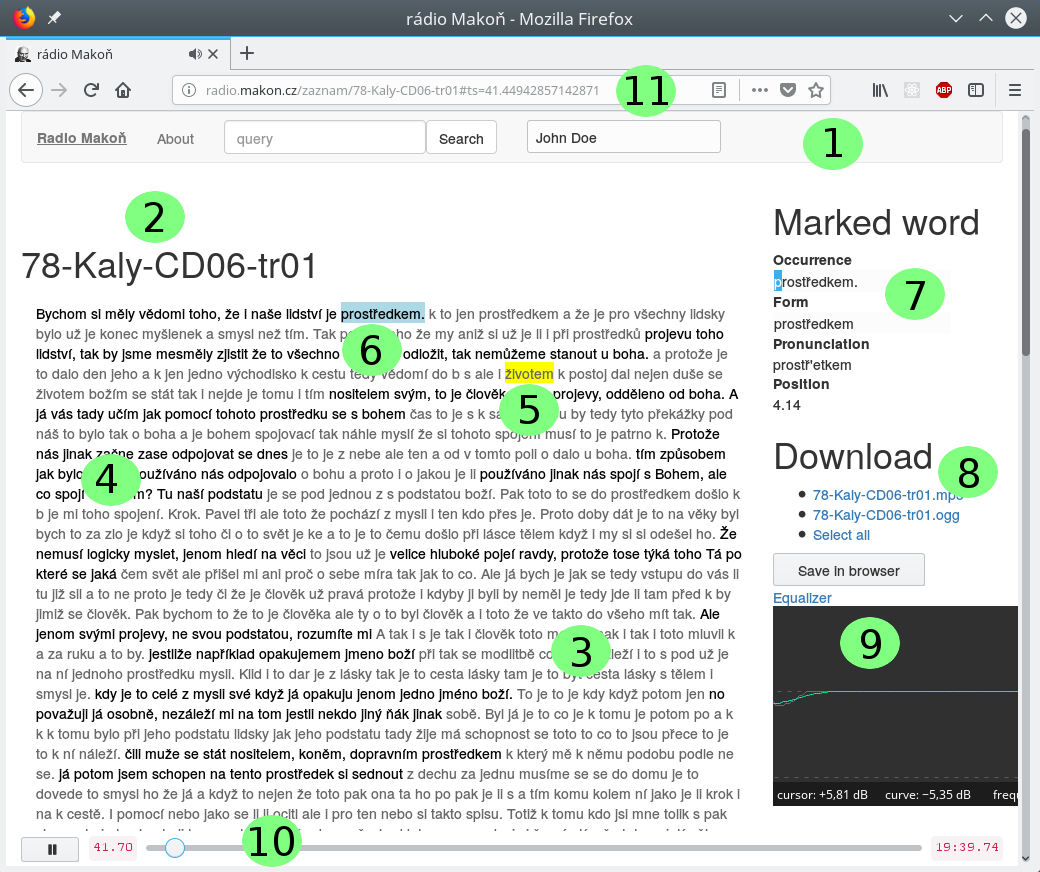
\includegraphics[scale=0.6]{rc/radio-makon-en-1-lab.png}
\caption{Web interface during playback}
\label{fig:scn1lab}
\end{figure}

Legend to Figure~\ref{fig:scn1lab}:
\begin{enumerate}
\item{
    Header with
    \begin{itemize}
    \item{app name linking to start page,}
    \item{about link,}
    \item{search field and}
    \item{username input field;}
    \end{itemize}
}
\item{Identifier of the recording;}
\item{Automatically transcribed segments in grey;}
\item{Manually transcribed segments in black;}
\item{Currently played-back word highlighted by yellow background;}
\item{Marked word highlighted in regent st. blue;}
\item{
    Marked word info:
    \begin{itemize}
    \item{
        occurrence: the word with contextual capitalization and
        punctuation as it appeared in the text (currently being edited as the
        selected initial letter reveals),
    }
    \item{form: normalized word form as it appears in the word list,}
    \item{pronunciation: Czech phonetic transcription of the word,}
    \item{
        position: time of the beginning of the word in seconds from the
        start of the recording;
    }
    \end{itemize}
}
\item{
    Tools for storing:
    \begin{itemize}
    \item{direct links to the audio files,}
    \item{selecting the whole transcription for easy pasting,}
    \item{storing the decoded recording in the browser's IndexedDB;}
    \end{itemize}
}
\item{Graphical equalizer for compensating narrow-band noise;}
\item{
    Audio playback controls:
    \begin{itemize}
    \item{play/pause button,}
    \item{current playback position,}
    \item{playback scrollbar,}
    \item{total recording length;}
    \end{itemize}
}
\item{Current position reflected in URL fragment.}
\end{enumerate}

\begin{figure}[htpb]
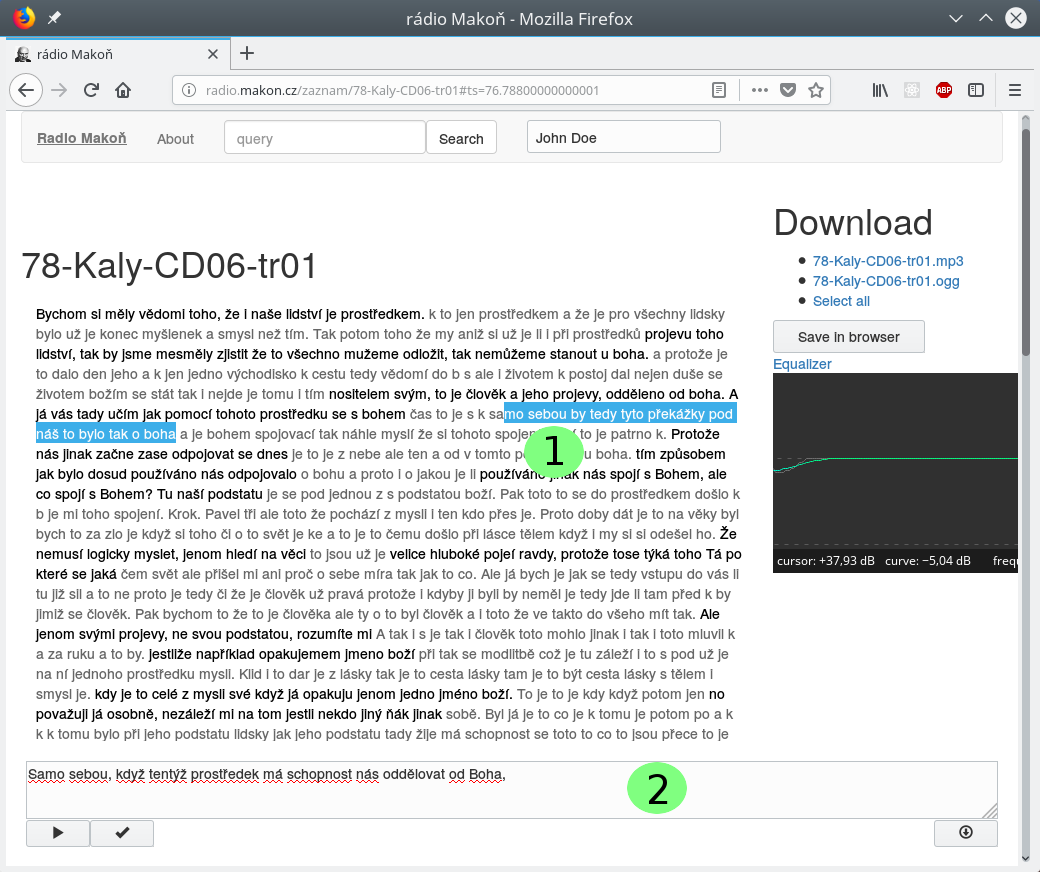
\includegraphics[scale=0.6]{rc/radio-makon-en-2-lab.png}
\caption{Interface in the state of editing a segment}
\label{fig:scn2lab}
\end{figure}

Legend to Figure~\ref{fig:scn2lab}:
\begin{enumerate}
\item{
    Selecting a text range with the mouse defines the segment the user is about
    to transcribe;
}
\item{
    The edit tool with
    \begin{itemize}
    \item{text area prefilled with the current transcription,}
    \item{playback button that plays the corresponding segment,}
    \item{save button and}
    \item{download-segment button, which initiates a file-save action for the
    audio segment corresponding the the selected text. The synthesis of the
    downloaded file takes place in the browser.}
    \end{itemize}
}
\end{enumerate}

The commonest tasks have keyboard shortcuts: \texttt{ctrl+space} for
play/pause and \texttt{ctrl+enter} for submitting a correction.

\subsection{Displaying the Transcription}

Many transcription programs show the transcription as a vertical list of
utterances, see Figure~\ref{fig:transcriber1} for an example of
Transcriber. We attribute this to the fact that the atomic elements of
the transcription are the user-entered utterances and their boundaries are
reliable. In our case, the atomic elements are words. There are sentences, sure,
but the segmentation to sentences by the ASR is very unreliable, so we want it
to be natural to transcribe a segment overlapping sentence boundaries.

\begin{figure}[htpb]
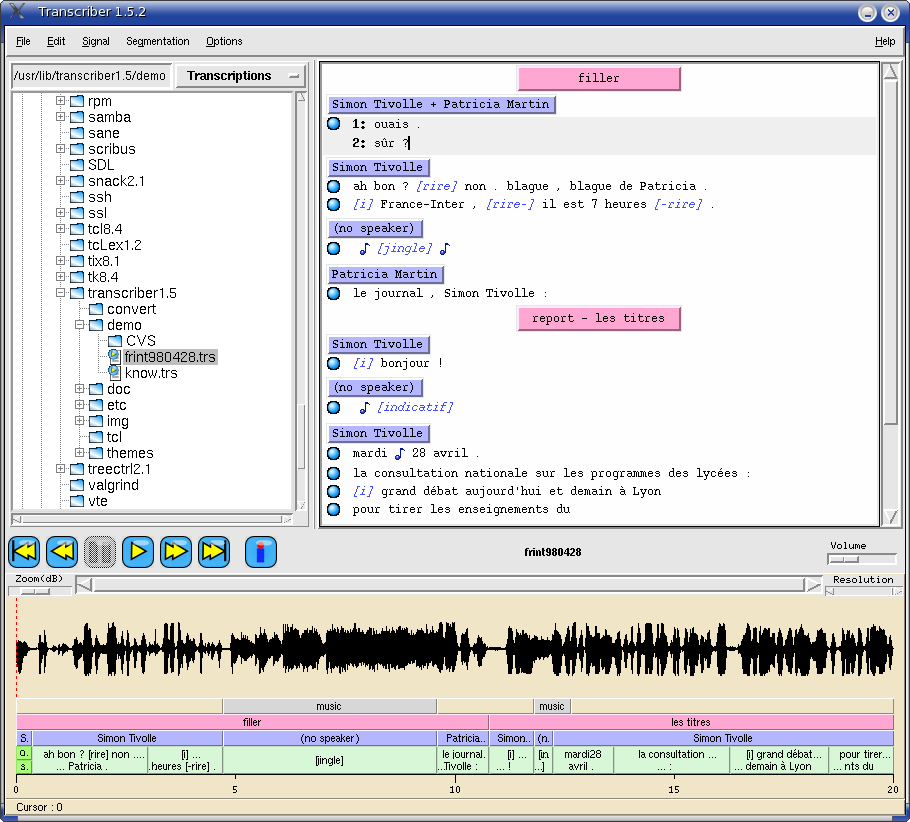
\includegraphics[scale=0.4]{rc/transcriber1.png}
\caption{A screenshot of Transcriber}
\label{fig:transcriber1}
\end{figure}

This is one of the reasons why we display the transcription basically as a
single wrapped line.

\subsubsection{Performance Challenge}

The transcription display was designed to have these features:
\begin{enumerate}
\item{
    Currently played-back word should be highlighted;
    \label{feats:item:curword}
}
\item{
    Manually transcribed segments should be clearly distinct from automatically
    transcribed ones;
    \label{feats:item:manualdistinct}
}
\item{
    Selecting one or more words with the mouse should trigger transcription mode
    for the selected text;
    upon a successful save, this should be merged into the display;
    \label{feats:item:selectable}
}
\item{
    Clicking a word should bring up its context info (we call this the
    {\em marked word} as the term {\em selected word} is already taken);
    \label{feats:item:clickable}
}
\item{
    The whole transcription should be shown at once for easy searching;
    \label{feats:item:showall}
}
\item{
    The page should be responsive.\label{feats:item:speed}
}
\end{enumerate}

These requirements are harder to combine than it may seem. Notably
responsiveness is hard to combine with all of the other ones. Why is that so?

Points~\ref{feats:item:curword} through \ref{feats:item:clickable}
call for every word to be wrapped in its own element.
Point~\ref{feats:item:showall} and the median count of words in a transcript of
about 6000 yield 6000 \texttt{<span>} elements just to show the text. 

Although this may not seem like a big deal, it does affect the responsiveness
and memory footprint of the page.

In the original version, we solved this by sacrificing point~5:
only 3 lines of text are shown with the current word kept on the middle line as
shown on Figure~\ref{fig:makonfm}.\footnote{The current word is on the top line
on the screenshot because it is at the beginning of the recording.} Thanks to
the development in the web standards and their support from popular browsers, a
solution is possible.

\begin{figure}[htpb]
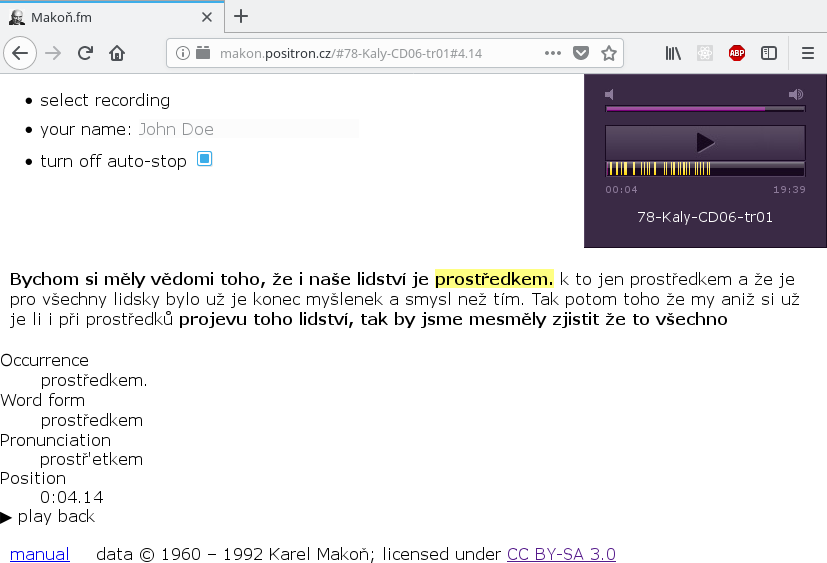
\includegraphics[scale=0.7]{rc/makonfm-en-1.png}
\caption{Original web interface from 2012}
\label{fig:makonfm}
\end{figure}

\subsubsection{Solution}

We can use the fortunate fact that manually transcribed words and automatically
transcribed ones tend to form larger chunks. The average number of words per
submitted segment is 7.9. Furthermore, the absolute majority of such segments
are adjacent to other manually transcribed chunks.\footnote{
The median number of chunks is 1 (most recordings have no manually corrected
segments), maximum is 1109. Median only counting touched recordings is 8.}
Hence, wrapping each chunk of consecutive manually or automatically transcribed
words in an HTML element is no problem, which solves
point~2.

Point~\ref{feats:item:selectable} can be implemented using
\texttt{document.selection} and the \texttt{Range} objects, which let us find
out the innermost HTML element and text offset of the start and end of the
textual selection. Since we know the length of each word, this allows us to map
the selection to the corresponding words in the transcription.

Points~\ref{feats:item:curword} and~\ref{feats:item:clickable} can be
implemented in two ways: We could either wrap the current and marked word in a
dedicated element or we could draw a highlighting rectangle beneath the word.

Wrapping the word would definetely be more robust and less error-prone but the
constant changes in the DOM during playback with possible frequent reflows speak
against it. Finding the exact position of each word and drawing a rectangle
precisely beneath it (beneath on the z-axis; over it in the x-y sense), avoiding
positioning issues and keeping the rectangle position synced even after scrolling
/ window resizing is definitely a challenge but we chose this way nonetheless.
The performance gain for the majority of the usage time outweighs the possible
errors in the corner cases, more so since the eventual errors are not critical
and mostly remedied by further playback.

The efficiency of repositioning a rectangle is supported by the fact that we can
calculate the coordinates of all rendered words once and only recalculate them
in two cases: 1) In the rare event of screen resize and 2) when a corrected
segment is merged into the transcription, in which case we only need to
recalculate for the words further in the document.\footnote{We could even stop
the recalculation as soon as we find that the new horizontal coordinate of a
word is left untouched, and add the difference in the vertical coordinate to all
subsequent words, i.e. when a line stays the same, so do all below it.}

\subsubsection{Manual / Automatic Distinction}

As shown on Figure~\ref{fig:scn1lab}, we draw automatic transcription in grey
and manual one in black. Why did we choose this instead of normal / boldface?
Firstly, the normal font is optimal for reading. Boldface is meant to highlight
spots in text. It becomes bulky when applied on long continuous passages. The
automatic transcription contains many errors, so there is no sense in optimizing
it for best reading experience.

There is also another practical reason. When the two font variants only differ
in color, and a segment of automatic transcription is left intact and submitted
as correct transcription, its merge-down into the displayed text causes no
reflow, which saves us computations and raises responsiveness. It may seem like
a rare use case but we believe that identifying correctly recognized words is a
legitimate way of contribution, so why not optimize for it?

Still, the underlying HTML tags are \texttt{<span>} and \texttt{<b>} because
that way the distinction persists when copy-pasting the text from the web page
to a rich text editor.

\subsection{Ergonomy}

It is clear that the ease of use is crucial in our case where the user is
supposed to perform a requiring, tedious task with repeated steps, especially
since it is our interest more than hers that she performs them. We compared our
setting with that of transcription apps in section~\ref{ssec:diff:trans},
pointing out lessons to learn. Let us now look at some specific points and their
actual (lack of) implementation.

\subsubsection{Keyboard Shortcuts}

One of the most profound measures in ergonomy are keyboard shortcuts. The most
common task is pausing and resuming playback. Both oTranscribe and Transcribe
use the \texttt{esc} key for that, and Transcriber uses the \texttt{tab} key.
We chose \texttt{ctrl+space} combination. We argue that \texttt{esc} is not the
best of options for desktops because the distance the fingers have to travel
from the alphanumeric keys causes a noticeable delay. This can lead to missing a
pause between words. The \texttt{tab} key as chosen by Transcriber is a splendid
choice from the ergonomy point of view and there is no reason not to use it in a
dedicated user interface. However, in the browser, where the \texttt{tab} key
has as native use, re-binding it could lead to confusion and irritation. The
space bar is probably the easiest-to-find key in all situations and dedicating
\texttt{ctrl} to all application-specific commands as opposed to single keys
lends a sense of consistency, we believe.

This is mere personal experience though, as we had no resources so far to
perform serious research to support these statements.

The only other keyboard shortcut we support is \texttt{ctrl+enter} for
submitting the correction. We chose this to stay consistent using the
\texttt{ctrl} key and because this shortcut is familiar to users of many instant
messengers, like the Facebook chat or the once popular official ICQ client.
Also, requiring a key combination prevents accidental submission, which is
desirable as we only want double-checked, guaranteed-precise ones. In
comparison, Transcriber uses the bare \texttt{enter} key to separate utterances.
oTranscribe and Transcribe allow free formatting with no explicit alignment, so
using the enter key to split utterances by lines is the user's choice.

\subsubsection{Missing Features}

One of the features that Transcribe, the only commercial tool in our reference
list, offers is setting up keyboard shortcuts for common words. We have not
implemented this because ideally, common words should be covered by speech
recognition. However, it could be sensible to implement it anyway. The reason is
that a word can be very rare globally and thus poorly recognized by ASR but very
common in a specific passage. This particularly regards named entities.

Another point in our ergonomy to-do list is lifting the need to select a segment
prior to correcting it. If the transcription was simply editable, it could
increase the ease of use rapidly. We would have to automate the selection of
segment to send for forced alignment but we could probably do a better job than
the user in the end.

\subsection{Mechanics of Submitting a Corrected Segment}

As stated above, when the user selects at least one character with the mouse,
the application enters the state of correcting the selected transcription padded
to whole words. In this mode, the transcription to correct is shown in a
text area and the global playback controls are replaced by those that only allow
playback of audio corresponding to the selected transcription.

Once the user believes that the content of the text area corresponds precisely
to the words uttered, she hits the {\em save} button or the \texttt{ctrl+enter}
keyboard shortcut. This starts an asynchronous HTTP request to the back-end,
where parametrized (MFCC) versions of the recordings are stored, along with the
new transcription and the time positions of the beginning and end of the
segment.

The server then cuts off the corresponding segment from the parametrized
recording, runs forced alignment on it with the provided transcription with a
threshold to reject bad matches. If the forced alignment fails, an error
response is sent back and the transcription is not merged into the original. In
the case of a success, the correction is merged on one hand on the server side
and pushed to a CDN, on the other hand it is merged into the transcription word
array in the JavaScript application. This redundancy warrants that we do not
have to reload the whole transcription every time a segment is corrected.

React ensures the updating of the chunks, and the coordinates of the words
further in the document are recalculated for word-highlighting purposes.

Apart from this, the version of the transcription to the recording is updated.
This is because the transcription files have a long cache time because normally,
they do not change at all. At the page load, the versions of all transcriptions
are loaded and used as cache busters. This enables us to use an external CDN and
cache effectively.

\subsection{Implementation Details}

\subsubsection{Audio Engine}

The adoption of Web Audio API\cite{adenot2013web} allowed for big improvements
in comparison with the original implementation. There are four major differences
between using the HTML \texttt{<audio>} tag and the Web Audio API.

\begin{itemize}
\item{It is now possible to precisely replay the selected audio span.}
\item{
    We could implement a graphical equalizer. Some recordings suffer from loud
    noise in the low frequency spectrum. A systematic approach to acoustic
    normalising of the material is a point of future work. Until that, the
    equalizer is a huge relief for the users.
}
\item{
    Thanks to the \texttt{OfflineAudioContext}, it is possible to store the
    recording in the browser's storage and avoid downloading or decoding it
    again after reload. We use \texttt{IndexedDB} as the storage method because
    \texttt{localStorage} has too low quota of about 10MB and the
    \texttt{FileSystem API} is not yet widely enough supported.
}
\item{
    We have also implemented saving the audio corresponding to the selected text
    segment as a sound file.
}
\end{itemize}

\subsubsection{App State Management}

We use React as the view library and Redux\cite{abramov2015redux} for state
management. The good thing about Redux is that it makes it easy to keep minimal
state as the single source of truth and everything that can be computed is
computed, while avoiding needless calculations. This is of course nothing new --
basically it is what we know from database design as the normal
representation\cite{codd1970relational}. It is the first time this approach
reached the web front-end in such degree of popularity though.

Also in our case, this approach makes the program more predictable, less
error-prone and, as the modern programming jargon lovingly expresses, {\em
easier to reason about}. But some of our features make this a bit complicated.

Among the states the app can enter is simple playback, inspecting a word and
transcribing a segment. The only relevant things we actually keep in the
Redux store are:

\begin{enumerate}
\item{
    The array of transcription words, each of which bears the flag whether it is
    automatically or manually transcribed. This defines the manual - automatic
    chunks of words that in turn define the HTML elements wrapping them.
}
\item{
    The beginning and end of the selection in terms of chunk number and
    character offset in the chunk, which is basically what we get from the DOM
    upon a \texttt{mouseup} event.
}
\end{enumerate}

Whether a word is marked or a segment is being edited is determined solely by
the boundaries of the selected words. If there is a selection and the beginning
and end are identical, it means a word was simply clicked and its detail is
shown (it is {\em marked}). If the boundaries span at least one character, then
all words that intersect this span are {\em selected} for correction.

Simple as it sounds, a slight problem arises when a correction is accepted and
the corrected subtitles are merged into the view. In the time after the
correction is accepted and reflected in the redux state, but before the new
chunks are rendered in the document, selection changes cannot be reliably mapped
to logical chunks. Simple null defaults solve this problem.

\section{Future Work}

We plan to focus on optimizing the app for wider audience. Experience confirms
that Mako\v{n}'s talks are of interest to some people, and our aim is to
remove as many obstacles as possible from potentially interested people reaching
the material. The benefit from technical point of view would be clear: A web app
for listening to recordings and correcting their transcription is nice but one
that is really easy to use and inviting to people to submit corrections is nicer.

One of the aspects we want to explore is enabling people to naturally share
catching segments of talks on social networks.

Another point of near-future endeavor is higher-level work with the contents. By
this we mean that we would like to use both automatic processing methods and the
users to do semantic analysis of the talks: What topic is covered where? What
topics are covered at all? Which talks relate to which written works?, and
similar questions.

We shall also deploy the technology on a different data set once we find a good
fit.

\section{Conclusion}

With our web application, a user can listen to recorded speech, see its
transcription with the currently played word highlighted, commit corrections to
the transcription, and inspect a word. The corrections are checked by a
forced-alignment mechanism on the server side. Our solution overcomes
performance challenges and is a serious improvement from the original version.
All our codebase is open-source, accessible on
Github\footnote{https://github.com/sixtease/MakonReact} and we are actively
looking for similar datasets with communities to employ the application on.

\section*{Acknowledgments}

The research was supported by SVV project number 260 453.\\
\\
This work has been using language resources stored
and distributed  by the LINDAT/CLARIN project of the Ministry of Education,
Youth and Sports of the Czech Republic (project LM2015071).

\bibliographystyle{splncs03}
\bibliography{citace}

\end{document}
